\documentclass{article}
\usepackage[utf8]{inputenc}
\usepackage[margin=1in]{geometry}
\usepackage[numbers]{natbib}
\usepackage{graphicx}
\usepackage{amsmath}
\usepackage{amssymb}
\usepackage[parfill]{parskip} % new line between paragraphs, no indentation
\usepackage[colorlinks,pdfstartview=FitH,citecolor=blue]{hyperref}

% Header
\usepackage{fancyhdr}
\pagestyle{fancy}
\fancyhf{}%Clear all heads and foots
\setlength{\headheight}{35pt} %Eliminate the warning of "headheight is too samll"
\rhead{Spatial Interpolation Methods\\Jianzhao Bi\\\today}
\cfoot{\thepage}

\begin{document}
Different methods can produce quite different spatial representations and in-depth knowledge of the phenomenon is needed to evaluate which one is the closest to reality. Quantitative evaluation of interpolation predictive capabilities, for example by cross-validation, is often not sufficient for the selection of an appropriate interpolation method, as the preservation of geometrical properties is in some cases more important than actual accuracy.

\begin{figure}[h!]
    \centering
    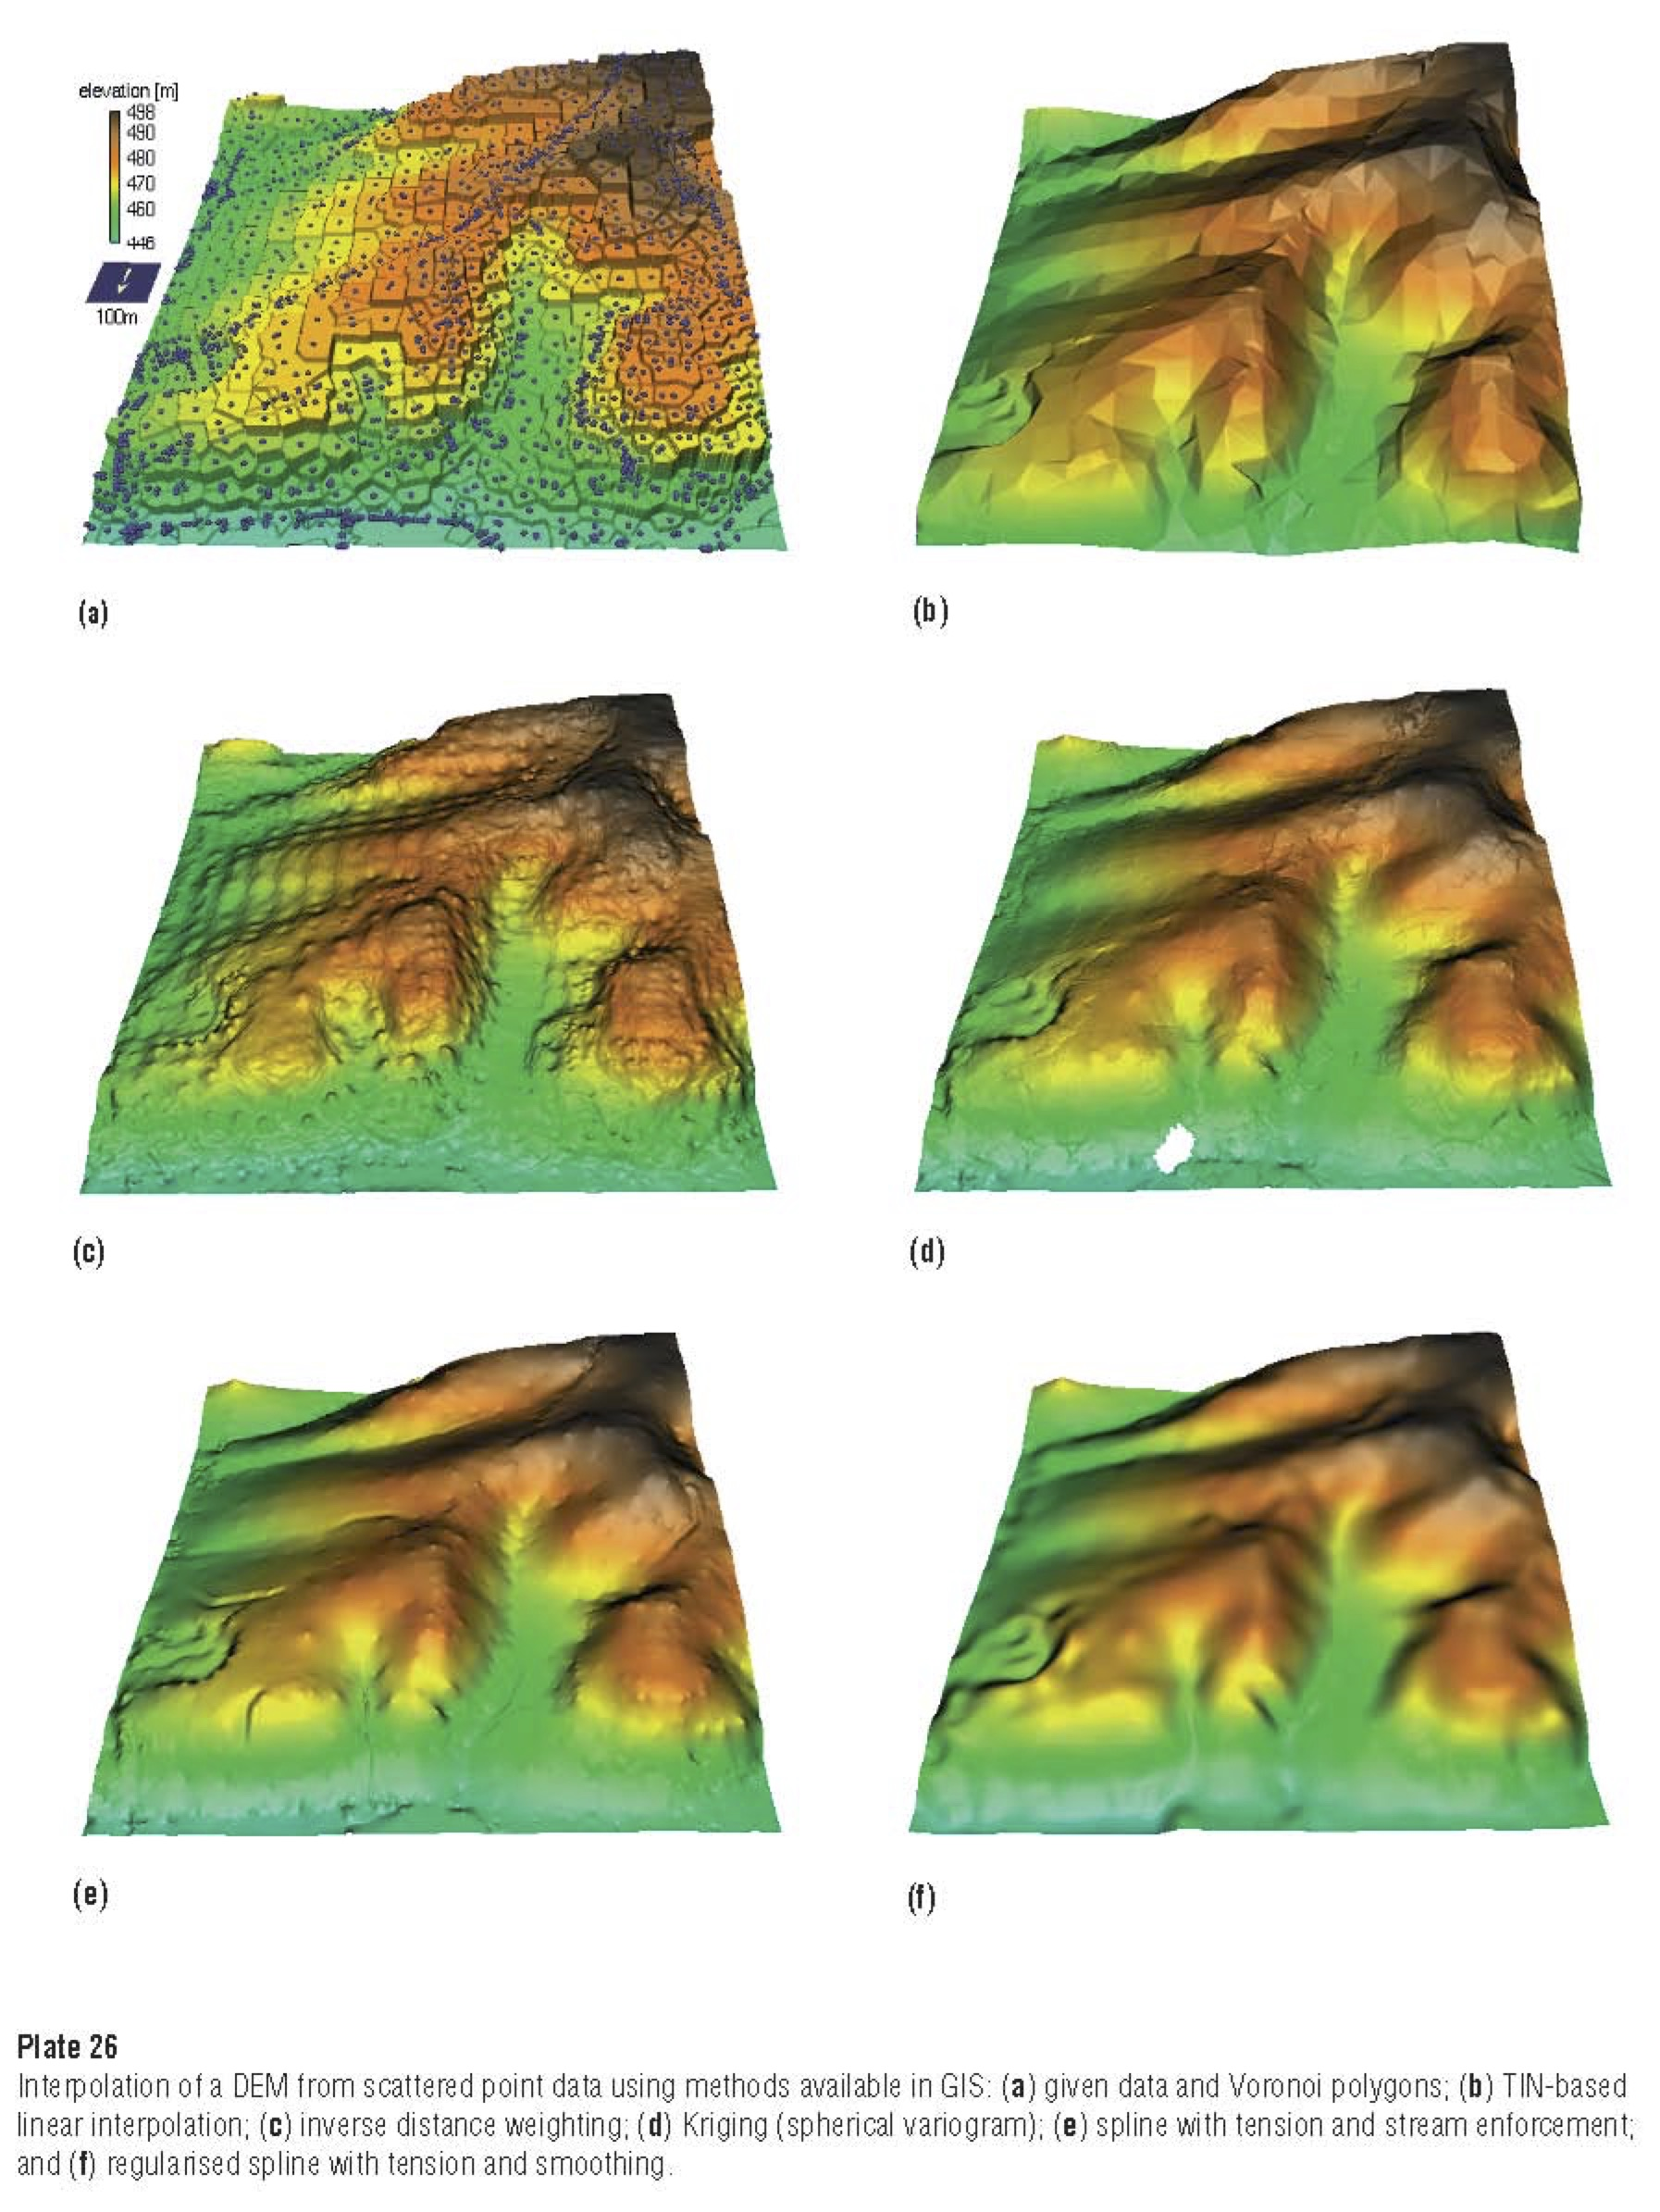
\includegraphics[width=0.65\textwidth]{img/interpolation.jpg}
    \caption{Different interpolation methods}
    \label{fig:my_label}
\end{figure}

\section{Local neighbourhood approach}
Local methods are based on the assumption that each point influences the resulting surface only up to a certain finite distance.
\paragraph{Inverse distance weighted interpolation (IDW)}
It is based on an assumption that the value at an unsampled point can be approximated as a weighted average of values at points within a certain cut-off distance, or from a given number of the closest points (typically 10 to 30). Weights are usually inversely proportional to a power of distance. However, the method often does not reproduce the local shape implied by data and produces local extrema (goose bumps) at the data points (Fig. \ref{fig:my_label}(c)).

\paragraph{Natural neighbour interpolation}
This uses a weighted average of local data based on the concept of natural neighbour coordinates derived from Thiessen polygons. The value in an unsampled location is computed as a weighted average of the nearest neighbour values with weights dependent on areas or volumes rather than distances. Natural neighbour linear interpolation leads to a rubber-sheet character of the resulting surface.

\paragraph{Interpolation based on a triangulated irregular network (TIN)}
This uses a triangular tessellation of the given point data (Boots, Chapter 36) to derive a bivariate function for each triangle which is then used to estimate the values at unsampled locations. While a TIN provides an effective representation of surfaces useful for various applications, such as dynamic visualization and visibility analyses, interpolation based on a TIN, especially the simplest, most common linear version, belongs among the least accurate methods 

\section{The geostatistical approach}
Kriging is based on a concept of random functions: the values in a surface are assumed to be the realizations of a random function with a certain spatial co-variance. The interpolated surface is then constructed using statistical conditions of unbiasedness and minimum variance. 

The main strengths of Kriging are in the statistical quality of its predictions (e.g. unbiasedness) and in the ability to predict the spatial distribution of uncertainty. 

It has been less successful for applications where local geometry and smoothness are the key issues and other methods prove to be competitive or even better: 1) subjective decisions are necessary (Journel 1996) such as judgment about stationarity, choice of function for theoretical variogram, etc. 2) often the data simply lack information about important features of the modelled phenomenon, such as surface analytical properties or physically acceptable local geometries. 

As mentioned earlier, Kriging is the most successful for phenomena with a very strong random component or for estimation of statistical characteristics (uncertainty).

\section{The variational approach}
The variational approach to interpolation and approximation is based on the assumption that the interpolation function should pass through (or close to) the data points and, at the same time, should be as smooth as possible. The variational approach offers a wide range of possibilities to incorporate additional conditions such as value constraints, prescribed derivatives at the given or at arbitrary points, and integral constraints.

However, most of the surfaces or volumes are neither stochastic nor elastic media, but are the result of a host of natural (\textit{e.g.,} fluxes, diffusion) or socioeconomic processes. Therefore, each of the mentioned methods has a limited realm of applicability and, depending on the knowledge and experience of the user, proper choice of the method and its parameters can significantly improve the final results. 

\section*{References}
\begin{itemize}
    \item Spatial interpolation: \url{https://www.geos.ed.ac.uk/~gisteac/gis_book_abridged/files/ch34.pdf}
\end{itemize}

\end{document}